\documentclass[10pt,letterpaper]{article}

\usepackage{amsmath}

\usepackage[T1]{fontenc} 
\usepackage[utf8x]{inputenc}
\usepackage[spanish]{babel}
\usepackage{graphicx}% Include figure files
\usepackage{blindtext} 

\usepackage{fancyvrb,xcolor}
\usepackage{upquote,textcomp}

%%% Margins
\oddsidemargin=-1.00cm
\textwidth=18.0cm
\topmargin=-2.54cm
\headheight=0cm
\headsep=2cm
\textheight=23.8cm


\usepackage{hyperref} % for urls


% Default fixed font does not support bold face
\DeclareFixedFont{\ttb}{T1}{txtt}{bx}{n}{8} % for bold
\DeclareFixedFont{\ttm}{T1}{txtt}{m}{n}{8}  % for normal

% Custom colors
\usepackage{color}
\definecolor{deepblue}{rgb}{0,0,0.5}
\definecolor{deepred}{rgb}{0.6,0,0}
\definecolor{deepgreen}{rgb}{0,0.5,0}
\definecolor{deepgray}{rgb}{0.5,0.5,0.5}

\usepackage{listings}

\lstdefinestyle{myCustomPythonStyle}{
	language=Python,
	basicstyle=\linespread{1}\small,
	otherkeywords={self},             % Add keywords here
	keywordstyle=\ttb\color{deepblue},
	emph={MyClass,__init__},          % Custom highlighting
	emphstyle=\ttm\color{deepred},    % Custom highlighting style
	commentstyle=\ttm\color{deepgray},
	stringstyle=\color{deepgreen},
	frame=tb,                         % Any extra options here
	showstringspaces=false,
	columns=fullflexible,
	keepspaces=true,
	literate={-}{-}1,				% To avoid problems with hyphen -
}



\makeatletter 
  \renewcommand\verbatim@font{\normalfont\ttfamily\color{blue}}
\makeatother


\title{ScientoPy - User Manual}


\begin{document}

% To fix ' no curve quotation mark
\newcommand\upquote[1]{\textquotesingle#1\textquotesingle}



\begin{tabular}{p{1.3in}p{6in}}
\begin{flushleft}
\noindent 
\includegraphics[bb = 2.5cm 0cm 10.29cm 9.78cm,scale=0.2]{./figures/escudoUnicacuaSolo.eps}
\end{flushleft} &
\normalsize \vspace{0.6cm}
\textsc{Universidad del Cauca}

\textsc{Facultad de Ingeniería Electrónica y Telecomunicaciones}

%\textsc{Maestría en Ingeniería Telemática}
\textsc{Programa de Ingeniería Electrónica y Telecomunicaciones}

%\textsc{Desarrollo de aplicaciones para plataformas ubicuas}

\textsc{ScientoPy, Installation and User Manual}

\end{tabular}
\begin{tabbing}
\hspace{3cm} \= \hspace{5.3cm} \= \hspace{6cm} \kill
\textbf{By}: \> Juan Pablo Ruiz Rosero			\> \texttt{jpabloruiz@unicauca.edu.co} \\
\end{tabbing}


\section{Installation}

\begin{enumerate}
\item Download and install the last version of Python 2.7 (for example Python 2.7.14) from: \\ \url{https://www.python.org/downloads/}
\item Install the  numpy, scipy, and matplotlib  libraries for Python with the automatic installation tool \textbf{pip}. From Windows, enter in the command line (Windows + R, cmd, and Enter), and run the installation script:
\begin{verbatim}
python -m pip install --user numpy scipy matplotlib
\end{verbatim}
\end{enumerate}


\section{Download the bibliometric dataset}
This section describes how to download the proper dataset from Scopus and WoS. Define a search criteria, it will be used for Scopus and WoS. For this guide we are using: "Internet of thing"  AND  "Gateway" 

\subsection{Download the dataset from Scopus}
\begin{enumerate}
\item Make your search with the defined search criteria for Article title, Abstract, Keywords. 
\item Select all the results and click on Export:
	\begin{center}
		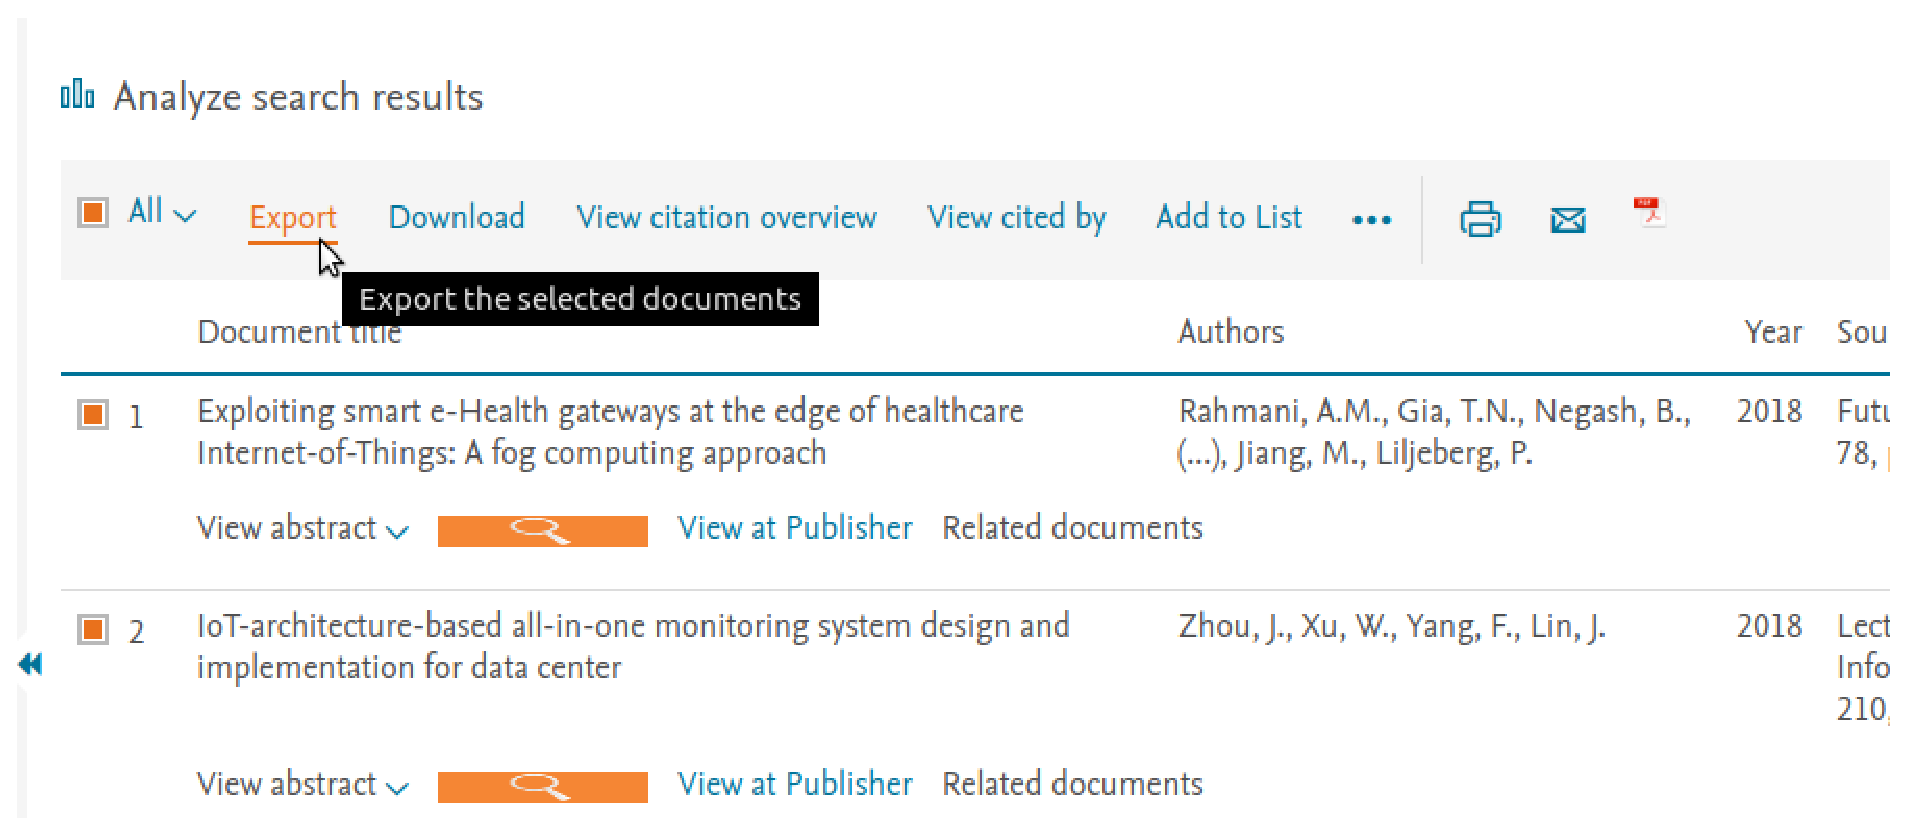
\includegraphics[scale=0.33]{./figures/scopus1.eps}
	\end{center}

\item Select as method of export \textbf{CSV (Excel)}, and select the Customize export \textbf{Citation information, Bibliographical information, Abstract and Keywords}, then click on Export: 
	\begin{center}
		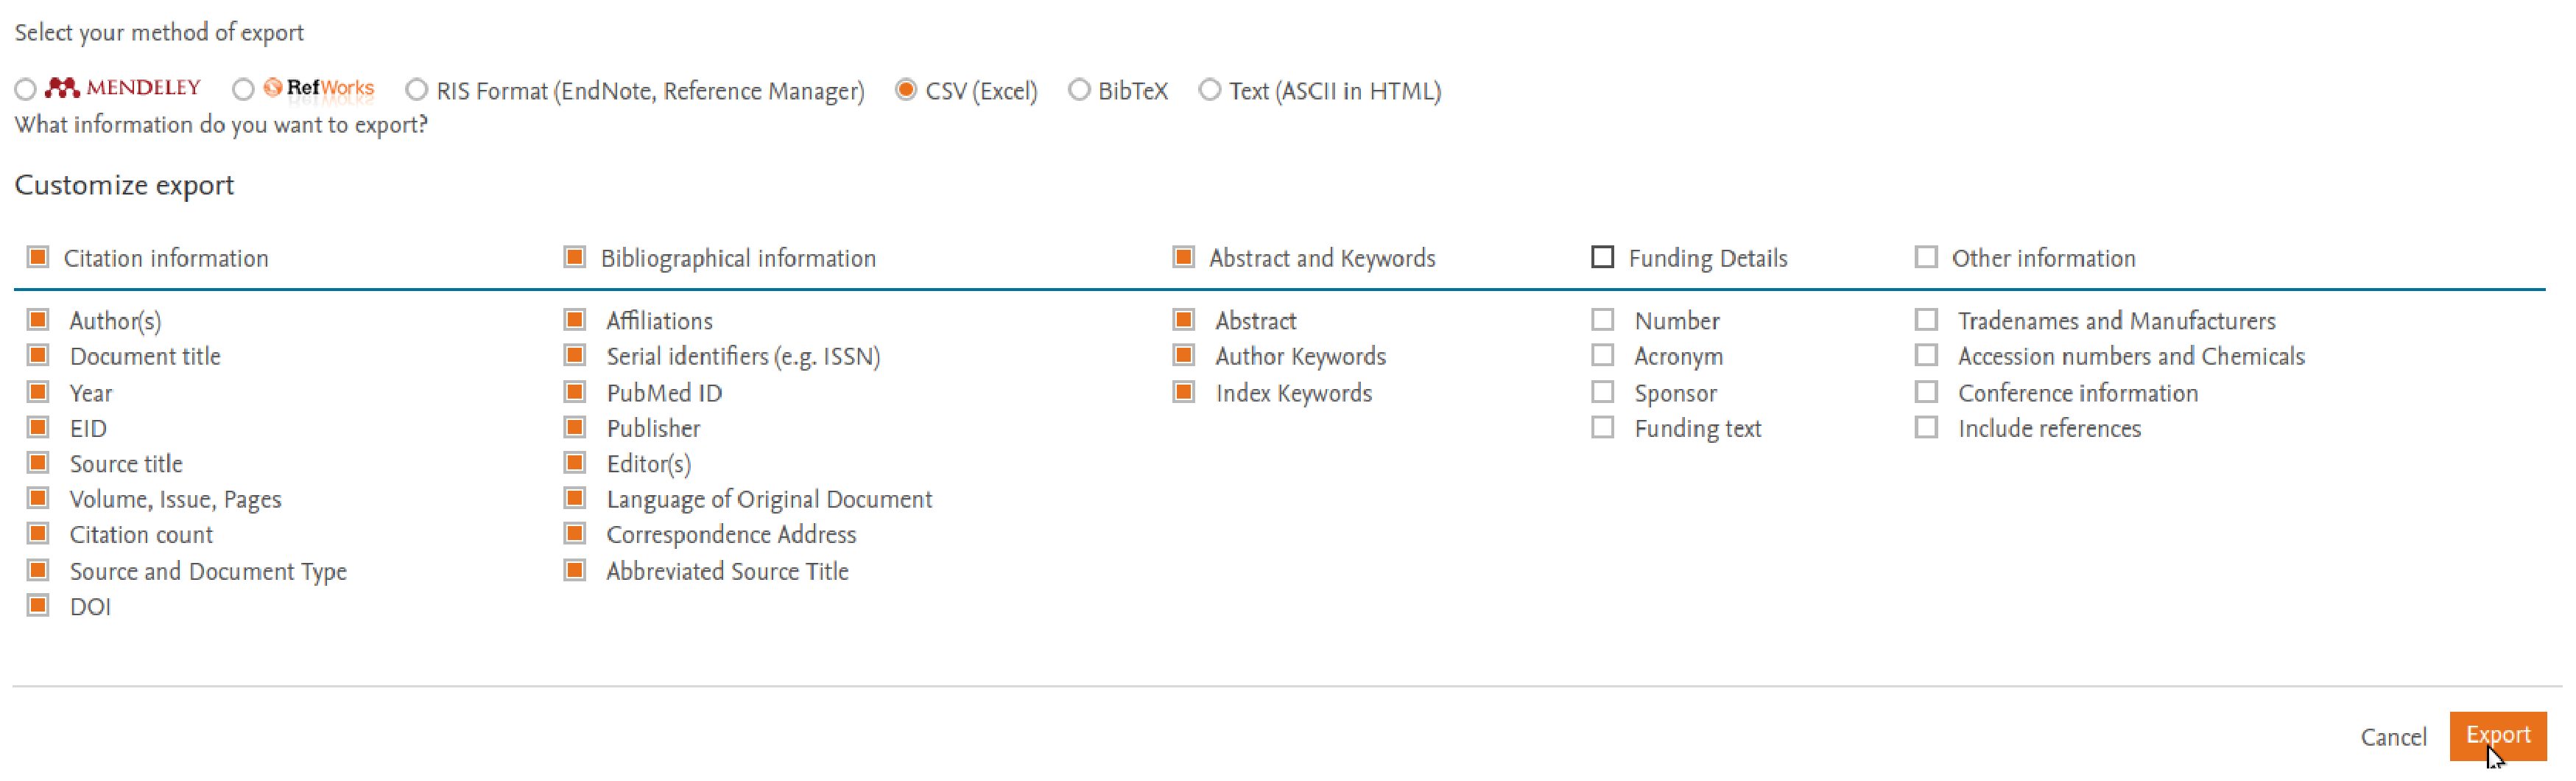
\includegraphics[scale=0.3]{./figures/scopus2.eps}
	\end{center}

\item Save the file on the folder \verb|/ScientoPy/dataIn|
\end{enumerate}


\subsection{Download the dataset from WoS}
\begin{enumerate}
\item Make your search with the defined search criteria for Topic. 
\item Select \textbf{Save in Other File Formats}
	\begin{center}
		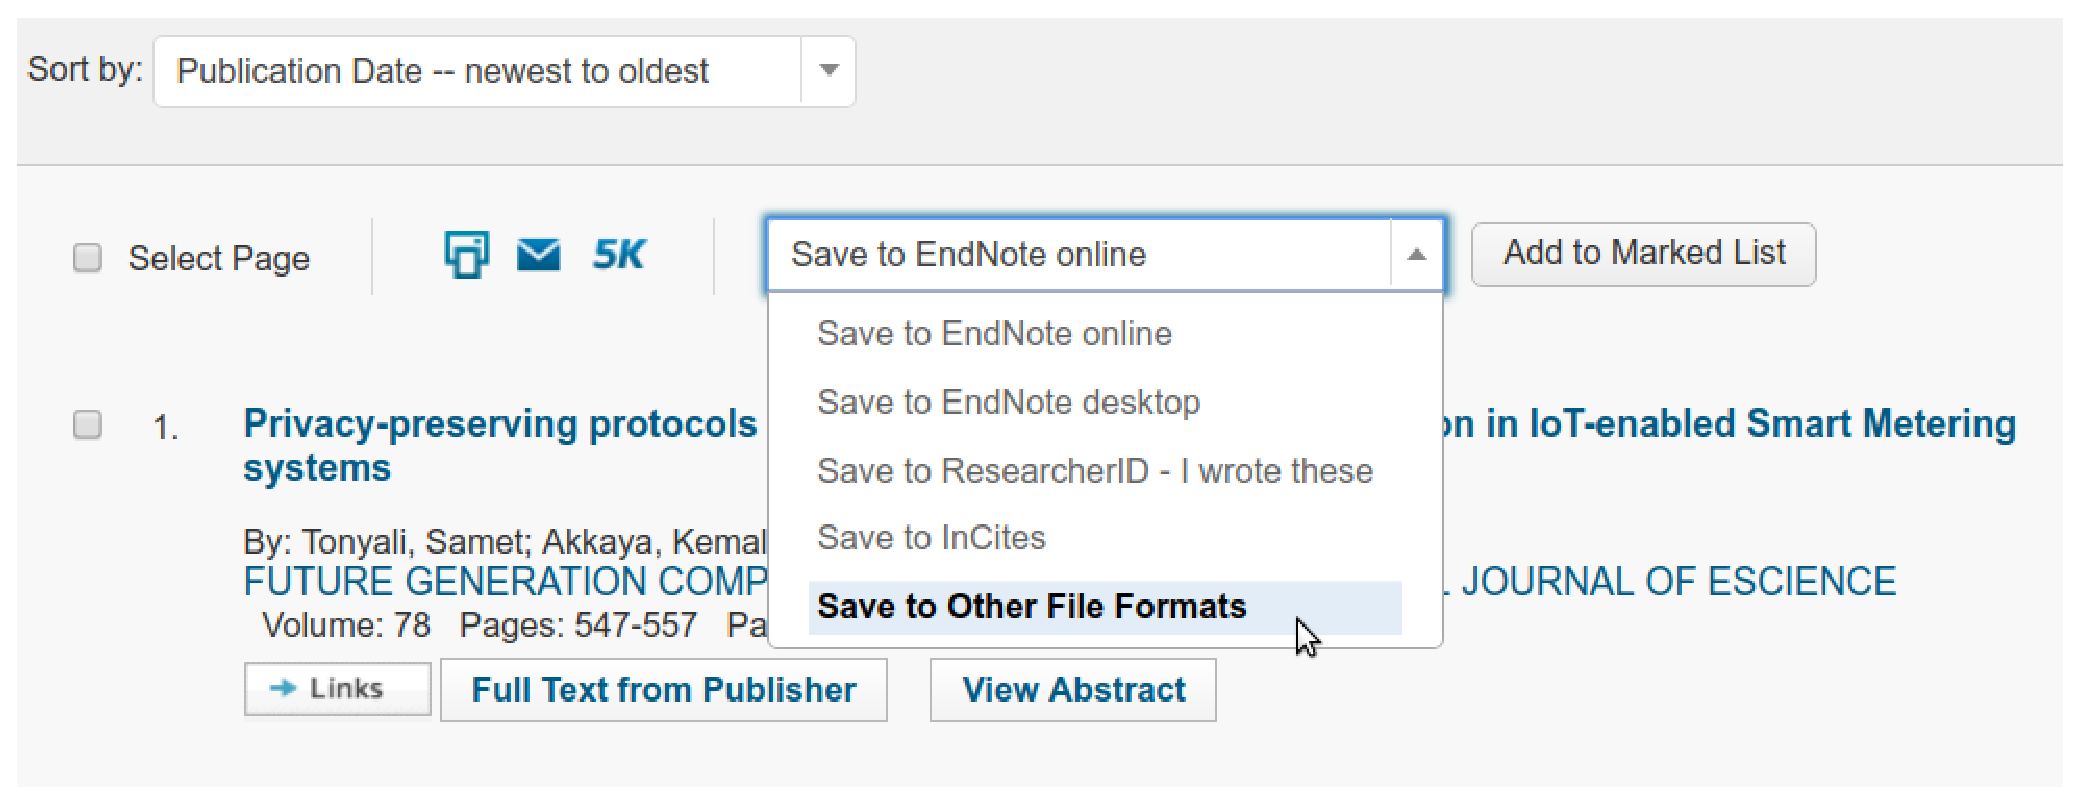
\includegraphics[scale=0.33]{./figures/wos1.eps}
	\end{center}

\item Select the number of records to download, on Record Contented select \textbf{Full Record and Cited References}, on File Format select \textbf{Tab-delimited (Win, UTF-8)}, and click on Send.
	\begin{center}
		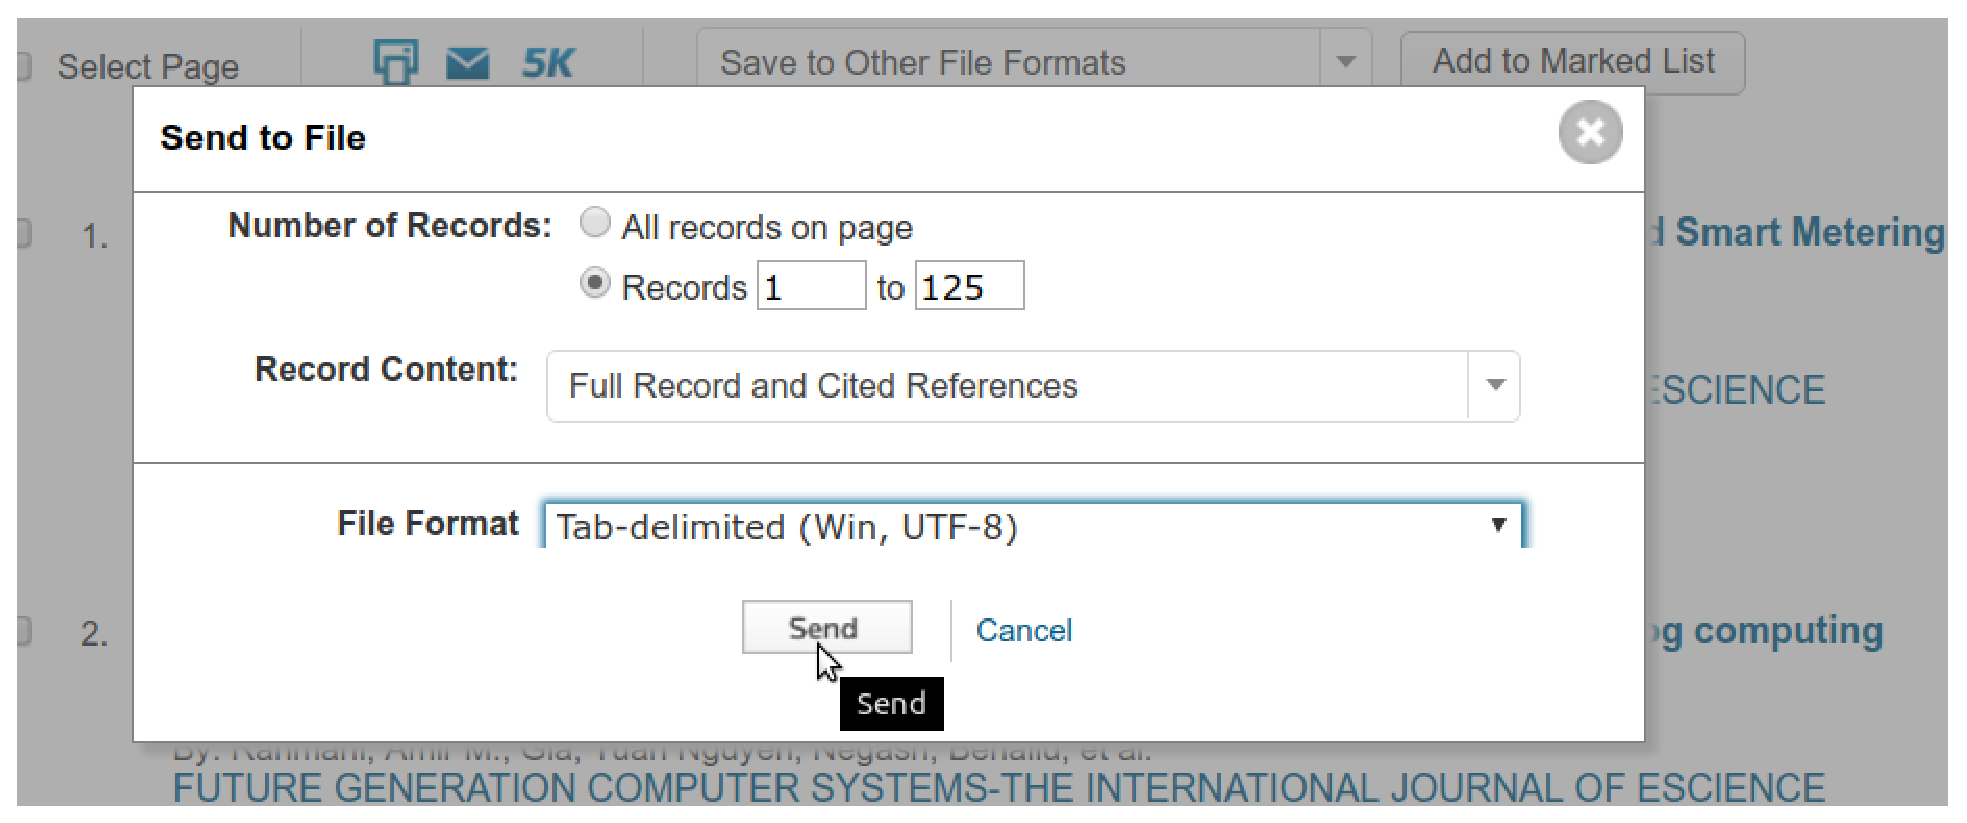
\includegraphics[scale=0.33]{./figures/wos2.eps}
	\end{center}

\item Save the file on the folder \verb|/ScientoPy/dataIn|
\end{enumerate}

\section{Running the ScientoPy scripts}

This section describes the ScientoPy scripts to pre-process and process the bibliometric dataset. 

\subsection{Pre-processing}

First we need to pre-process the downloaded dataset. This pre-process joint all the downloaded files from one folder to a single file. Also, this process remove the duplicated files. To pre-process the example dataset (Internet of things papers) run this command inside ScientoPy folder: 
\begin{verbatim}
python preProcess.py dataInIoT
\end{verbatim}

Then, inside the folder \verb|ScientoPy/dataPre| you will find the following files: 
\begin{itemize}
\item \textbf{papersPreprocessed.csv:} this file contains the information of all papers after the pre-process. This file will be used by the others scripts as the input data. 
\item \textbf{PreprocessedBrief.csv:} this file briefs the pre-process statics results, such as duplicated papers removed, types of documents, and others. 
\end{itemize}

To find more options of the pre-processing script you can run:
\begin{verbatim}
python preProcess.py -h
\end{verbatim}

\subsection{Extract the top topics}

With this script you can extract the top topics of a selected criterion. The ScientoPy script criteria are:

\begin{itemize}
\item authors
\item source
\item subject 
\item authorKeywords 
\item indexKeywords 
\item documentType 
\item dataBase 
\item country
\item institution
\end{itemize}

For example, to find the top author's keywords you can run this script: 

\begin{verbatim}
python scientoPy.py authorKeywords
\end{verbatim}

This will generate a list with the top 10 topics on the selected criterion (in this case authorKeywords), with the number of documents per topic, and the h-index associated to each one. Also, this script graphs the evolution of each topic per year, and saves the quantitative results on the folder \verb|ScientoPy/results|. 

This script have more options like, save the plot on a file, or increase the number of topic results. For more information you can run:

\begin{verbatim}
python scientoPy.py -h
\end{verbatim}

\subsection{Analyze pre-defined topics inside a criterion}

If you want to make an analysis of pre-defined topics, such as the two selected countries papers evolution, you can use the \verb|scientoPy.py| script, with the option \verb|-t|, to specify the topics: 

\begin{verbatim}
python scientoPy.py country -t "United States; Brazil"
\end{verbatim}

You can analyze any topic in any criterion. Put the topics on the \verb|-t| argument. Divide the topics with the \verb|;|. Also, you can integrate two or more topics in one, by dividing it with \verb|,|. This is very useful for abbreviations and plural singulars, for example: 
\begin{verbatim}
python scientoPy.py authorKeywords -t \
"WSN, Wireless sensor network, Wireless sensor networks; RFID, RADIO FREQUENCY IDENTIFICATION"
\end{verbatim}

\textbf{Note: } The command is very long, for that reason the command was divided by "\". If you have problems in Windows, remove the "\" and put the command in one single line.

Also, you can see the results with a parametric graphic (add \verb|--parametirc|). This option plot the accumulative documents, average growth rate (AGR), and h-Index of the selected topic, for example:

\begin{verbatim}
python scientoPy.py authorKeywords -t \
"WSN, Wireless sensor network, Wireless sensor networks; RFID, RADIO FREQUENCY IDENTIFICATION" \
--parametric
\end{verbatim}

This script have more options like, save the plot on a file, or others. For more information you can run:

\begin{verbatim}
python scientoPy.py -h
\end{verbatim}

\subsection{Finding trending topics}

This script finds the top trending topics based on the higher average growth rate (AGR) over the others. The AGR is calculated on two years periods, using the following Equation \eqref{equation_AGR}:
\begin{equation}
AGR = \frac{\sum\limits_{i = Y_s}^{Y_e}P_i - P_{i-1}}{(Y_e - Y_s)+1},  
\label{equation_AGR}
\end{equation}
where:\\
$AGR$ = Average growth rate;
	
	$Y_s$ = Start year;
	
	$Y_e$ = End year;
	
	$P_i$ = Number of publications on year $i.$
\newline


To find the top trending topics on author's keywords criterion, you can run the following script: 

\begin{verbatim}
python trendResults.py authorKeywords
\end{verbatim}

This script will find the top 200 topics, then it calculates the AGR for the last 3 periods of 2 years. Finally, the 200 top topics are sorted from the highest AGR in the last 2 year period to the lower. The first 10 AGR topics with the corresponding value per period is graphed. 

Also, you can find the AGR for selected topics inside a criterion, writing the topic on the argument \verb|-t|, like the following example: 

\begin{verbatim}
python trendResults.py authorKeywords -t "Cloud computing;Security;Big Data"
\end{verbatim}

This script have more options like, save the plot on a file, get the list from the lower last period AGR to the higher, or others. For more information you can run:

\begin{verbatim}
python trendResults.py -h
\end{verbatim}


\subsection{Finding trending documents}

The trending documents are the new publications with more citations. To find these publications, this script scale the citations of each publication based on a Year Scale (YS). The YS put more weight to newer publications, by the following Equation \eqref{equation_YS}:
\begin{equation}
YS_i = e^{(i - Y_s)*Y_w}
\label{equation_YS}
\end{equation}
where:\\
$YS_i$ = Year scale for year $i$;
$i$ = Year;
$Y_s$ = Start year;
$Y_w$ = Year weight, default 1;
\newline

The number of citations (citat) of each document is multiplicated by the corresponding $YS_i$, to get the Scaled citations (S. cita). The final publications list is sorted by this Scaled citations. The following script find the trending documents as described:

\begin{verbatim}
python topCited.py
\end{verbatim}

This script, graphs the all documents citations sum per year, this citations sum scaled (multiplied by the $YS_i$), and the scale per year ($YS_i$). If you want to put more weight to the citation than publication year, you can reduce the Year weight. On the other way, if you want to put more weight to the newer papers you can increase the year weight. The recommended values are between 0 to 5. For example, to get the most cited document of the last years you can run the script with a Year weight of 1.75:

\begin{verbatim}
python topCited.py --yearWeight 1.75
\end{verbatim}


The full document list results is saved in the file \verb|ScientoPy/results/topCitedPapers.csv|. This script have more options like, save the plot on a file, or others. For more information you can run:

\begin{verbatim}
python topCited.py -h
\end{verbatim}

\end{document}  